\documentclass[10pt]{article}
\usepackage[margin=0.78in]{geometry}
\usepackage[T1]{fontenc}
\usepackage{lmodern,amsmath,amssymb,booktabs,graphicx,microtype,fancyhdr,longtable}
\usepackage[hidelinks]{hyperref}
\usepackage{xurl}
\pagestyle{fancy}\fancyhf{}\setlength{\headheight}{14pt}
\fancyhead[L]{\small HPS Gaussian-Process Resonance Search}
\fancyhead[R]{\small v6.3.1 / 2021 10\%}\fancyfoot[C]{\thepage}
\setlength{\parindent}{0pt}\setlength{\parskip}{5pt}
\setlength{\emergencystretch}{2em}\renewcommand{\arraystretch}{1.12}
\newcommand{\Ah}{\widehat A}\newcommand{\sh}{\widehat\sigma}
\hypersetup{pdftitle={HPS-GPR v6.3.1: 2021 10 percent fixed-yield injection study},pdfauthor={Emrys Peets}}
\begin{document}
\begin{center}{\LARGE Fixed-yield injection and recovery}\\[5pt]
{\large 2021 10\%: independent pilot, native MC and Gaussian signals}\\[4pt]
Emrys Peets\quad---\quad24 September 2026\end{center}

\section*{Result and scope}
The study completed all 80 evaluation cells with 100 attempted toys per cell: 8,000/8,000 valid signed free fits and 8,000/8,000 valid truth-fixed profiles. The independent pilot contains 2,000/2,000 valid fits. There are 0 unresolved fit/profile rows in the failure ledger. 
The same expected full-selected signal yield $A=z s_0(m)$ is used for both shapes and every evaluation toy at each mass and level. The Gaussian pilot mean returned yield error defines the frozen $s_0$; $z$ is an input reference-strength label, not an achieved significance.
At $z=5$, mean raw recovery ranges over the ten masses are 0.94--1.10 for Gaussian signals and 0.78--1.04 for native MC. Mean paired response, which subtracts each toy's matched null fit, ranges from 0.96--0.98 and 0.72--0.89, respectively. These ranges describe cells, not independent pooled measurements. The native-MC paired response is lower than the Gaussian response at every mass at $z=5$; the pointwise paired-difference intervals below quantify the difference. Equal expected candidate counts do not imply equal extraction difficulty.
\begin{center}\small\begin{tabular}{rcccccc}\toprule
& \multicolumn{2}{c}{Raw recovery} & \multicolumn{2}{c}{Paired response} & \multicolumn{2}{c}{Pull width}\\
$m$ [MeV] & Gaussian & MC & Gaussian & MC & Gaussian & MC\\\midrule

60 & 1.04 & 0.87 & 0.96 & 0.72 & 0.92 & 1.04\\

80 & 1.10 & 1.04 & 0.98 & 0.87 & 1.08 & 0.94\\

100 & 1.05 & 0.93 & 0.98 & 0.88 & 0.95 & 0.87\\

120 & 0.99 & 0.88 & 0.97 & 0.88 & 0.96 & 1.11\\

140 & 0.94 & 0.91 & 0.97 & 0.89 & 0.96 & 1.00\\

160 & 0.97 & 0.87 & 0.97 & 0.88 & 0.79 & 0.87\\

180 & 0.98 & 0.87 & 0.97 & 0.88 & 1.06 & 1.02\\

200 & 0.95 & 0.82 & 0.97 & 0.87 & 0.93 & 0.93\\

220 & 1.00 & 0.91 & 0.97 & 0.85 & 0.99 & 0.94\\

240 & 0.95 & 0.78 & 0.97 & 0.81 & 0.94 & 0.97\\

\bottomrule\end{tabular}\end{center}
{\small Summary at $z=5$. Recovery and response are averages of per-toy ratios. Full cell uncertainties and paired differences are supplied as CSV; figures below show standard errors. Pull width is the sample standard deviation, with $n-1$ denominator.\par}
This is a conditional study of one pinned background mean, fixed empirical MC templates and one archived-kernel GP prescription. It measures fixed-yield bias, error response and nominal signed profile-set containment. It does not establish physical-background adequacy, unconditional coverage, calibrated discovery significance or an exclusion.
\clearpage\section*{Ensemble and frozen reference}
Two disjoint cohorts each contain 100 full-support Poisson background spectra, sampled from the bundled nominal 2021 GP arithmetic mean. Each cohort reuses its backgrounds across all ten masses. Evaluation also reuses each background across both shapes and four levels. The 8,000 evaluation rows are therefore correlated across cells; they do not represent 8,000 independent background experiments.
\begin{align*}B^{\rm pilot}_{ji},B^{\rm eval}_{ti}&\sim\operatorname{Poisson}(b_i),&s_0(m)&=\frac1{100}\sum_{j=0}^{99}\sh^{\rm pilot}_{A,G,j}(m),\\A(m,z)&=z s_0(m),&S_{tmzi}&\sim\operatorname{Poisson}(A(m,z)w_i).\end{align*}
The full probability vector includes bins below and above analysis support. Signal is added in all analysis bins, including GP training sidebands. The realized full signal total fluctuates around $A$; expected and realized counts are recorded separately. Within each shape case, generation and extraction use identical full-selected-count probabilities. No fit-window or support renormalization is applied.
\begin{center}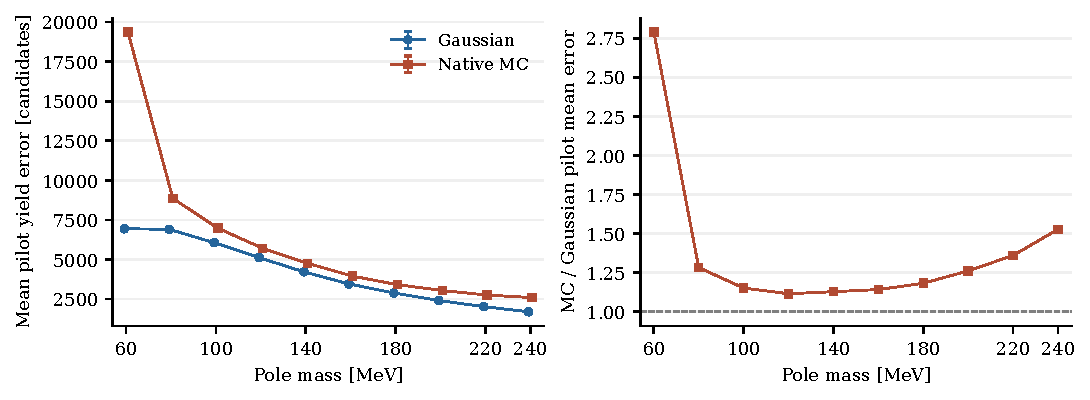
\includegraphics[width=\textwidth]{../figures/pilot_reference.pdf}\end{center}
{\small Pilot mean returned yield errors (left; bars are standard errors of the 100 pilot errors) and their MC/Gaussian ratio (right). The Gaussian mean alone defines the common frozen yield scale. The ratio panel is descriptive; its sampling uncertainty is not shown.\par}

\begin{center}\small\begin{tabular}{rrrrrr}\toprule$m$ [MeV] & $s_0$ & SE$(s_0)$ & Gaussian CV [\%] & MC/Gaussian & $A(z=5)$\\\midrule

60 & 6944.94 & 0.38 & 0.054 & 2.790 & 34724.72\\

80 & 6907.96 & 0.16 & 0.023 & 1.283 & 34539.78\\

100 & 6062.10 & 0.12 & 0.019 & 1.152 & 30310.49\\

120 & 5118.65 & 0.11 & 0.021 & 1.115 & 25593.27\\

140 & 4219.16 & 0.10 & 0.024 & 1.129 & 21095.81\\

160 & 3458.43 & 0.10 & 0.030 & 1.142 & 17292.15\\

180 & 2885.38 & 0.10 & 0.034 & 1.182 & 14426.90\\

200 & 2410.70 & 0.10 & 0.042 & 1.262 & 12053.48\\

220 & 2022.51 & 0.12 & 0.061 & 1.361 & 10112.54\\

240 & 1698.53 & 0.14 & 0.082 & 1.528 & 8492.66\\

\bottomrule\end{tabular}\end{center}
The pilot table is frozen before evaluation. Its standard error describes pilot precision; it is not added to a pull denominator or resampled during evaluation bootstraps.
\clearpage\section*{Raw recovery and paired response}
For every positive injection, two diagnostics retain different information:\[Q_t=\frac{\Ah_t(A)}{A},\qquad R_t=\frac{\Ah_t(A)-\Ah_t(0)}{A}.\]Raw recovery retains any background-only yield offset. Paired response subtracts the signed null fit of the same background, mass and extraction template. The subtraction is used only here; it is absent from raw yields, pulls and likelihood profiles.
\begin{center}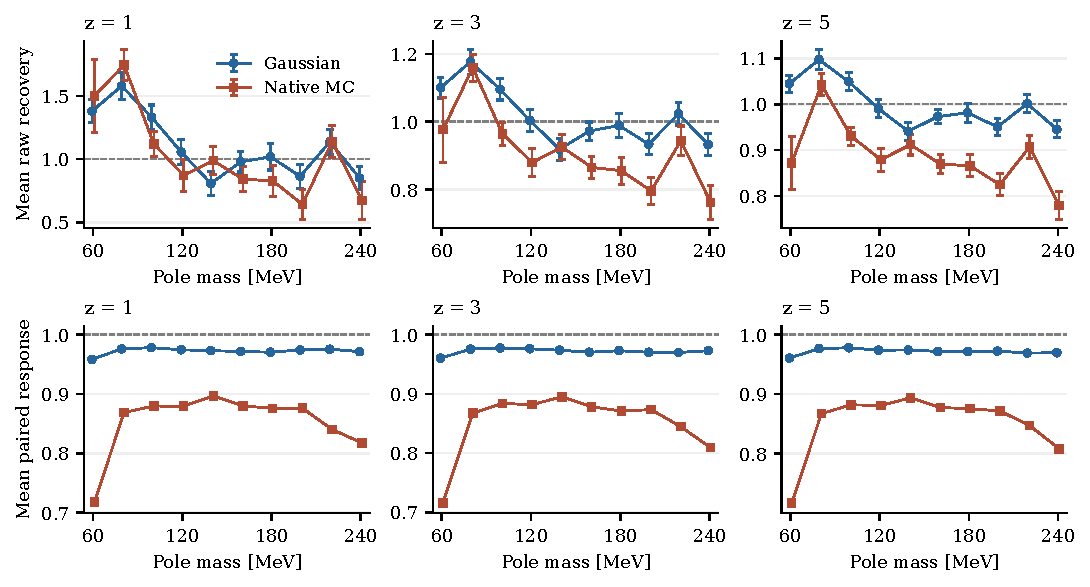
\includegraphics[width=\textwidth]{../figures/recovery.pdf}\end{center}
{\small Cell means with standard errors from the toy scatter. The dashed line denotes unit recovery/response. MC and Gaussian receive equal expected full-selected yields at each mass and level; their independent Poisson signal draws need not have equal realized totals.\par}

\subsection*{Paired MC--Gaussian response differences at $z=5$}
\begin{center}\small\begin{tabular}{rrrr}\toprule $m$ [MeV] & MC minus Gaussian & 95\% bootstrap interval & Complete pairs\\\midrule

60 & -0.244 & [-0.248, -0.241] & 100\\

80 & -0.109 & [-0.112, -0.107] & 100\\

100 & -0.096 & [-0.098, -0.094] & 100\\

120 & -0.093 & [-0.095, -0.091] & 100\\

140 & -0.081 & [-0.083, -0.078] & 100\\

160 & -0.094 & [-0.097, -0.092] & 100\\

180 & -0.096 & [-0.099, -0.093] & 100\\

200 & -0.101 & [-0.105, -0.097] & 100\\

220 & -0.122 & [-0.127, -0.118] & 100\\

240 & -0.162 & [-0.167, -0.157] & 100\\

\bottomrule\end{tabular}\end{center}
The whole-toy bootstrap uses the same resampled evaluation IDs in every cell and preserves null partners. Each difference uses complete MC/Gaussian pairs; missing pairs are disclosed in the machine-readable table. These are pointwise intervals without a multiple-comparison adjustment.
\clearpage\section*{Absolute bias and returned errors}
Absolute bias is $\overline{\Ah-A}$ in full-selected candidates. Returned-error response is the average of $\sh_A/s_0$. Neither the returned error nor $s_0$ is the empirical spread of fitted yields; the latter is saved separately as \texttt{Ahat\_sd}.
\begin{center}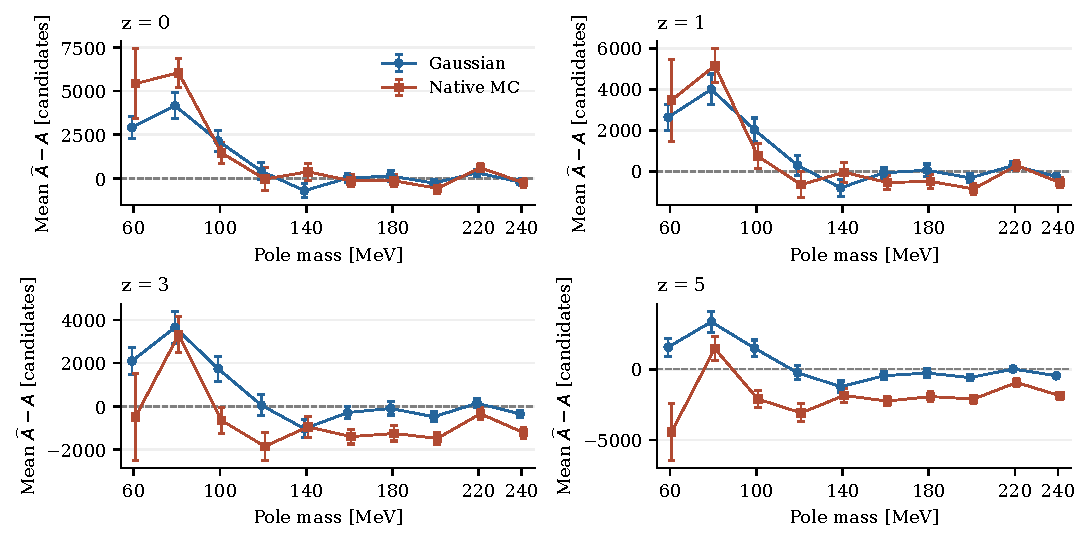
\includegraphics[width=\textwidth]{../figures/absolute_bias.pdf}\end{center}
{\small Mean absolute bias; bars are standard errors across valid fits. At $z=0$ these are the signed null offsets.\par}

\begin{center}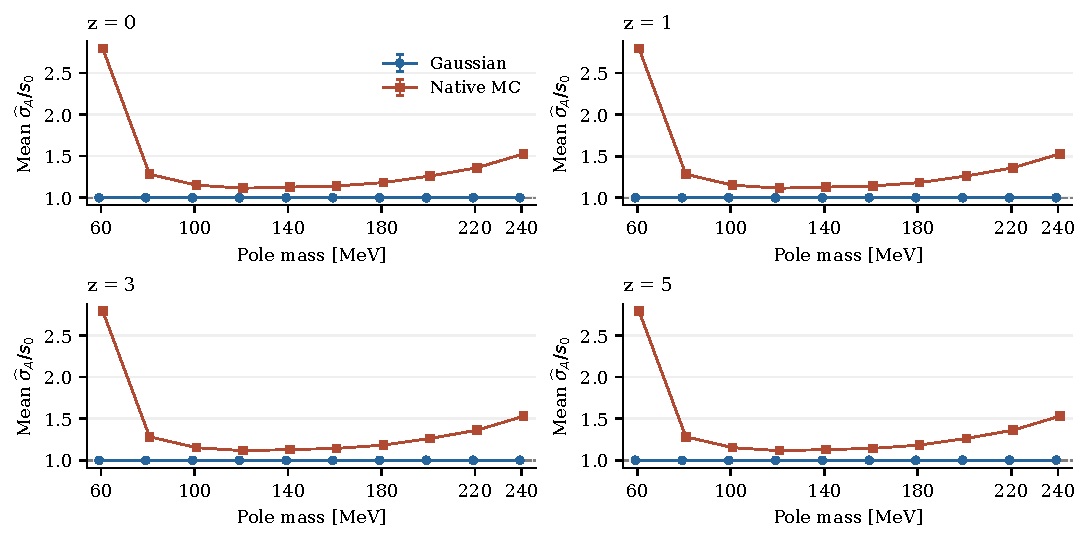
\includegraphics[width=\textwidth]{../figures/error_response.pdf}\end{center}
{\small Mean returned yield error divided by the frozen Gaussian reference. Bars are standard errors of the per-toy ratios. The dashed line is unity.\par}

\clearpage\section*{Pull location and width}
The primary pull uses the fixed expected yield and each fit's returned profile-Hessian uncertainty:\[p_t=\frac{\Ah_t-A}{\sh_{A,t}}.\]The realized Poisson signal total is not substituted for $A$. Unit pull width and zero pull mean are diagnostic reference values, not numerical acceptance criteria.
\begin{center}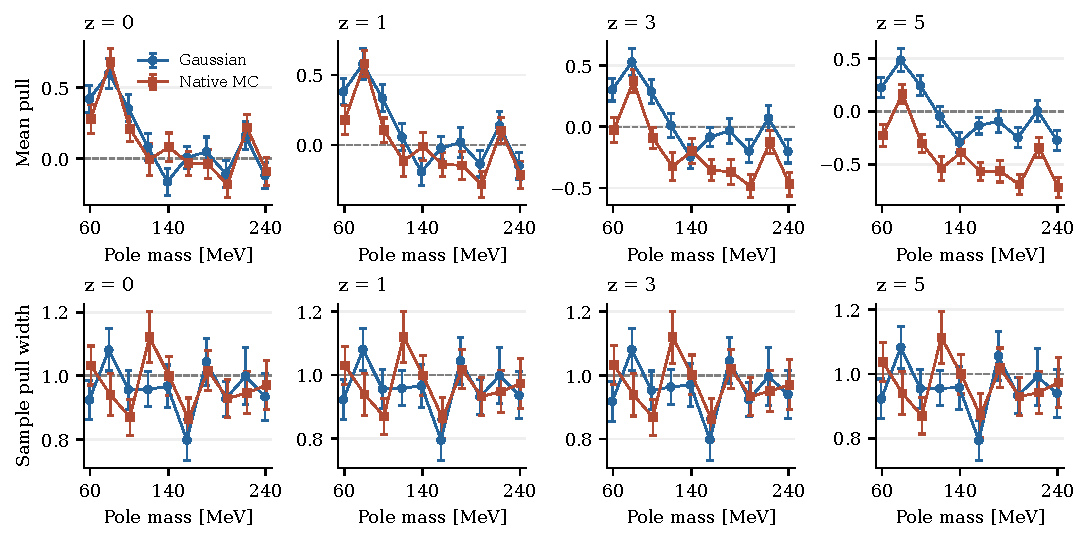
\includegraphics[width=\textwidth]{../figures/pulls.pdf}\end{center}
{\small Top: mean pull with toy-sample standard error. Bottom: sample pull width with one-standard-error whole-toy bootstrap bars (2,000 fixed-seed replicates). Dashed lines mark zero mean and unit width. The accompanying CSV includes pointwise 95\% percentile intervals for the widths.\par}

\subsection*{Null offsets cannot be removed by changing the injection scale}
At zero signal, each template may project the background residual differently. The null fits remain signed. Using a common expected yield changes the positive-injection ensemble; it does not alter either template's null bias.
\begin{center}\small\begin{tabular}{rcccc}\toprule & \multicolumn{2}{c}{Null mean pull} & \multicolumn{2}{c}{Null pull width}\\$m$ [MeV] & Gaussian & MC & Gaussian & MC\\\midrule

60 & 0.42 & 0.28 & 0.92 & 1.03\\

80 & 0.60 & 0.68 & 1.08 & 0.94\\

100 & 0.35 & 0.21 & 0.96 & 0.87\\

120 & 0.08 & -0.01 & 0.96 & 1.12\\

140 & -0.17 & 0.08 & 0.97 & 1.00\\

160 & 0.01 & -0.03 & 0.80 & 0.86\\

180 & 0.05 & -0.04 & 1.04 & 1.02\\

200 & -0.11 & -0.19 & 0.93 & 0.93\\

220 & 0.16 & 0.22 & 1.00 & 0.95\\

240 & -0.12 & -0.09 & 0.93 & 0.97\\

\bottomrule\end{tabular}\end{center}
\clearpage\section*{Nominal signed profile-set containment}
For each toy, nuisance coordinates are refitted at the fixed expected $A$, with the same GP mean/covariance used by that toy's free fit:\[q_{\rm true}=2\{\mathrm{NLL}(A,\widehat\theta_A)-\mathrm{NLL}(\Ah,\widehat\theta)\}.\]Truth is counted inside the nominal 68.27\% and 95\% signed profile-likelihood sets when $q_{\rm true}\leq1$ and $q_{\rm true}\leq3.841459$, respectively. These are signed sets, not a physical nonnegative-signal upper-limit construction.
\begin{center}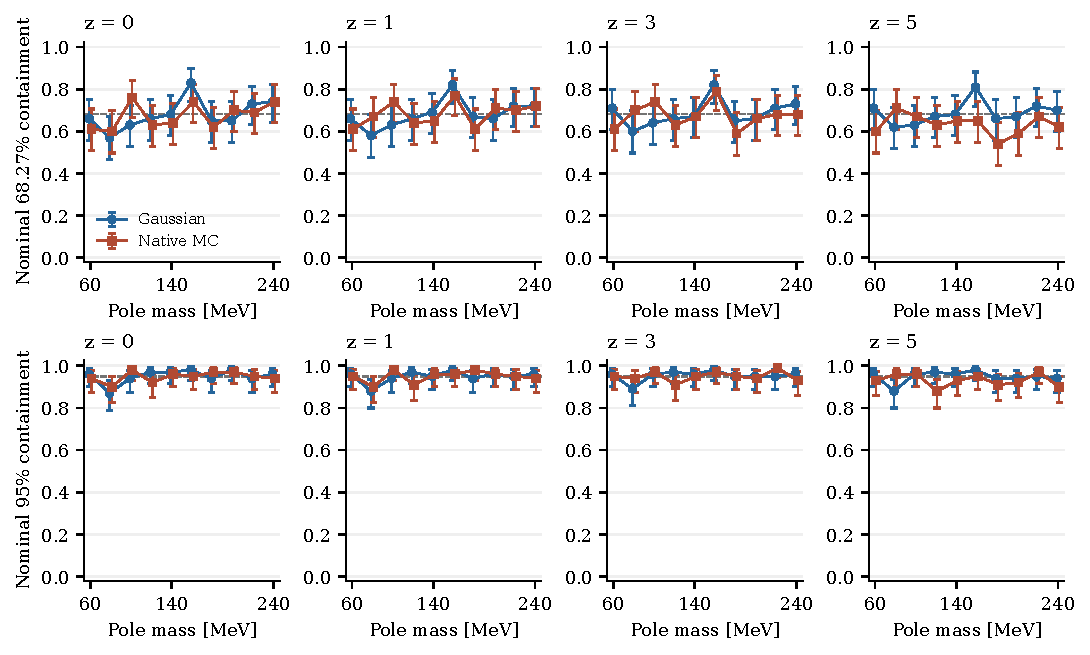
\includegraphics[width=\textwidth]{../figures/containment.pdf}\end{center}
{\small Containment among numerically valid truth profiles. Bars are exact 95\% Clopper--Pearson intervals using that cell's valid-profile denominator. Dashed lines show nominal reference levels. Shared backgrounds correlate the cells; the intervals are pointwise.\par}

\begin{center}\small\begin{tabular}{rrcccc}\toprule & & \multicolumn{2}{c}{68.27\% count range} & \multicolumn{2}{c}{95\% count range}\\$z$ & attempted/cell & Gaussian & MC & Gaussian & MC\\\midrule

0 & 100 & 57--83 & 60--76 & 87--98 & 90--98\\

1 & 100 & 58--82 & 61--77 & 88--98 & 90--98\\

3 & 100 & 60--82 & 59--79 & 89--98 & 91--99\\

5 & 100 & 62--81 & 54--71 & 88--98 & 88--97\\

\bottomrule\end{tabular}\end{center}
Ranges are over mass cells; they are not pooled proportions. Exact cell counts, denominators and intervals are in \texttt{evaluation\_summary.csv}. For $k$ containing profiles and $f$ unresolved decisions, all-attempt accounting bounds are $[k/100,(k+f)/100]$. These bounds are not confidence intervals. Successful-fit containment is conditional on numerical success; the failure ledger and valid fractions remain part of the result.
For this run, valid-profile denominators range from 100 to 100 out of 100. With only 100 toys per cell, percentage-level claims require the reported binomial uncertainty; the shared-cell design cannot be treated as additional independent precision.
\clearpage\section*{Representative spectra and GP response}
Representative spectra are selected by fixed toy ID and declared masses, without selection by fit quality or recovery. Full-support plots show the added signal tails; window and residual panels show the response of GP conditioning to the same injected spectrum. A plotted GP shift is a diagnostic, not a decomposition proving that every recovery difference arises from sideband absorption.
\subsection*{Gaussian signals}
\begin{center}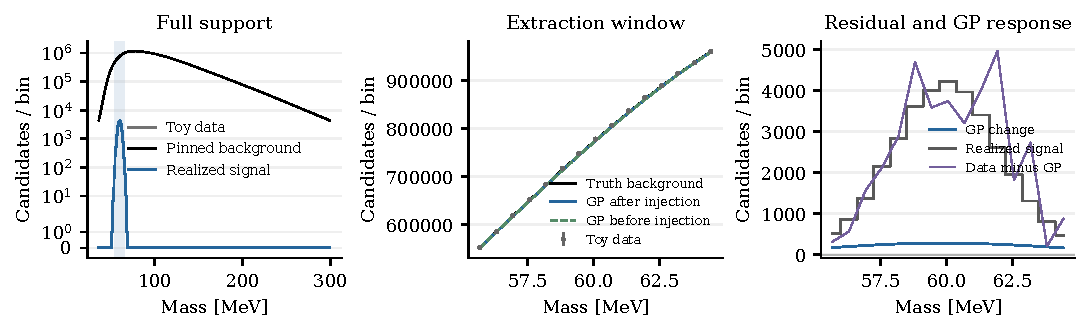
\includegraphics[width=\textwidth]{../figures/spectrum_m060_gaussian.pdf}\end{center}
{\small 60 MeV, Gaussian, $z=5$, evaluation toy 0. The green dashed curve is the matched background-only GP prediction.\par}

\begin{center}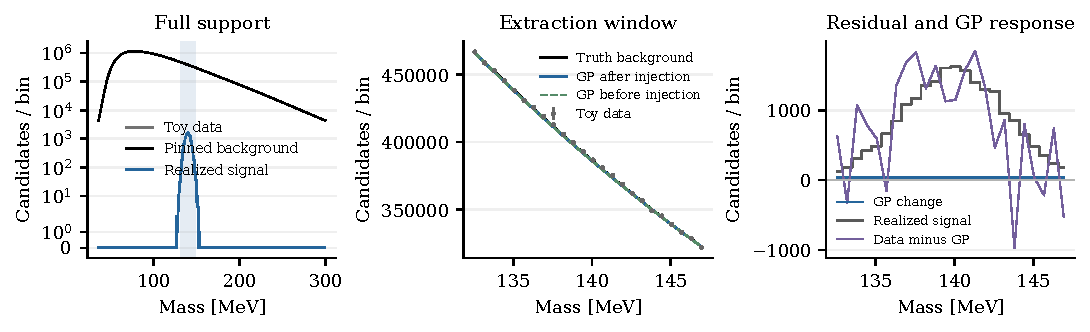
\includegraphics[width=\textwidth]{../figures/spectrum_m140_gaussian.pdf}\end{center}
{\small 140 MeV, Gaussian, $z=5$, evaluation toy 0. The green dashed curve is the matched background-only GP prediction.\par}

\begin{center}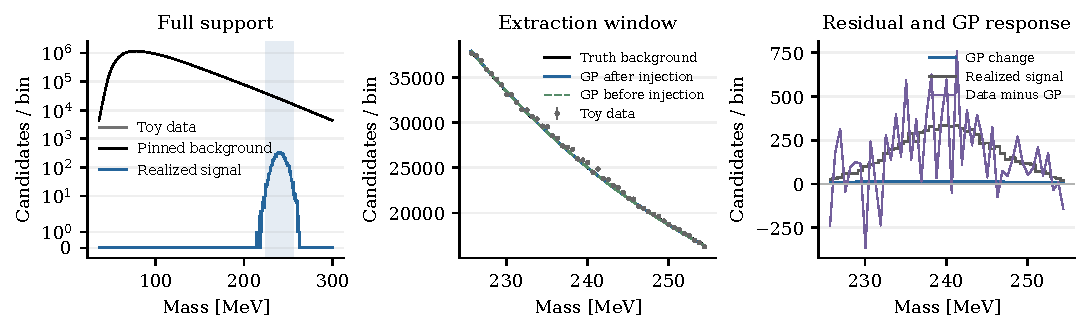
\includegraphics[width=\textwidth]{../figures/spectrum_m240_gaussian.pdf}\end{center}
{\small 240 MeV, Gaussian, $z=5$, evaluation toy 0. The green dashed curve is the matched background-only GP prediction.\par}

\clearpage\section*{Representative spectra: native MC}
The same evaluation background (toy 0), masses, pole-centered masks and common expected yields are used as on the Gaussian page. Signal draws are independent across shapes. The nominal native-MC template is used both to generate and fit these signals.
\begin{center}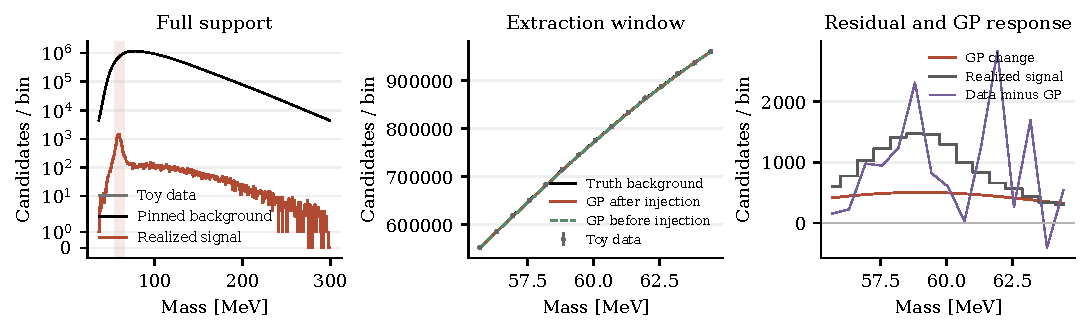
\includegraphics[width=\textwidth]{../figures/spectrum_m060_mc.pdf}\end{center}
{\small 60 MeV, Native MC, $z=5$, evaluation toy 0. The green dashed curve is the matched background-only GP prediction.\par}

\begin{center}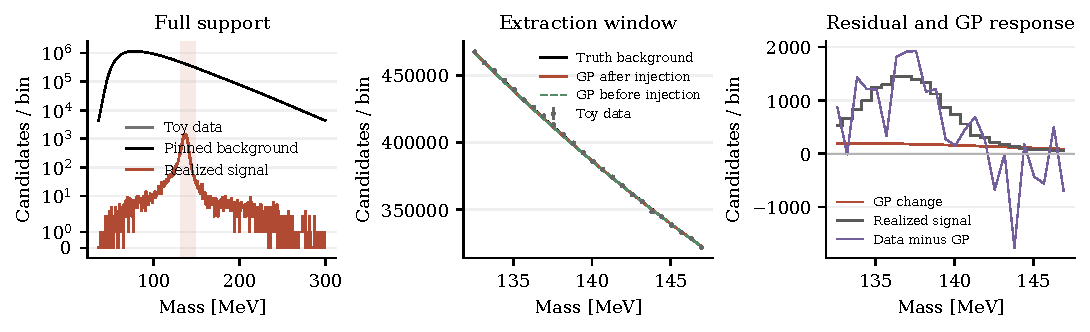
\includegraphics[width=\textwidth]{../figures/spectrum_m140_mc.pdf}\end{center}
{\small 140 MeV, Native MC, $z=5$, evaluation toy 0. The green dashed curve is the matched background-only GP prediction.\par}

\begin{center}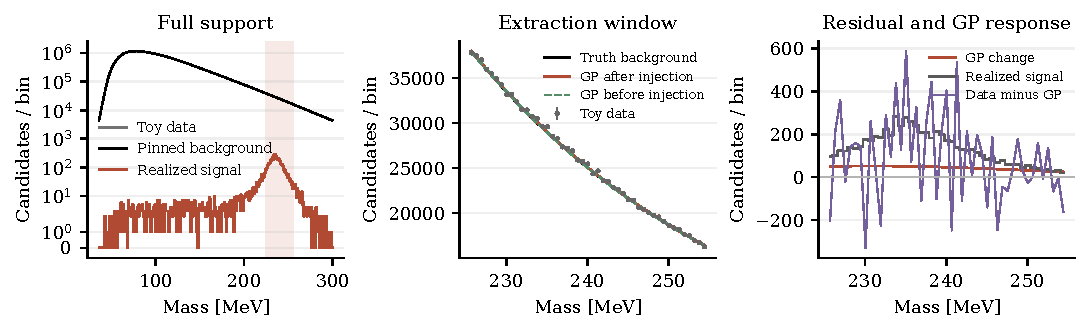
\includegraphics[width=\textwidth]{../figures/spectrum_m240_mc.pdf}\end{center}
{\small 240 MeV, Native MC, $z=5$, evaluation toy 0. The green dashed curve is the matched background-only GP prediction.\par}

Native MC and Gaussian differences can include core offset, width, tails and pole-centered window acceptance. This run does not isolate these components. Clean-sideband or model-mismatch controls would be separately specified diagnostics.
\clearpage\section*{Procedure, numerical accounting and provenance}
All masses use the pole-centered window $m\pm2.25\sigma_m$, with the same extraction and training masks for both shapes. The nominal resolution is $\sigma_m=0.00184825-0.001375m+0.085875m^2$, with $m$ and $\sigma_m$ both in GeV. Gaussian bin probabilities are CDF differences; native MC probabilities use the pinned histogram CDF with its inherited uniform-within-bin convention and outside-support categories.
The GP uses archived mass-dependent kernel parameters. Each spectrum recomputes its count-dependent log targets/noise, conditional mean and correlated covariance from bins outside the window. Positive counts use $\log n$ and noise variance $1/n$; zero counts use target zero and variance one. This is GP conditioning with fixed kernel parameters, without hyperparameter optimization. The inherited signed count-yield likelihood is\[\lambda_i=\widehat b_i+(L\theta)_i+A w_i,\qquad\mathrm{NLL}=\sum_{i\in W}(\lambda_i-n_i\log\lambda_i)+\tfrac12\theta^\top\theta.\]Poisson means remain positive. Returned uncertainties are observed profile-Hessian yield errors. Truth profiling holds the toy's GP constraint fixed, without further retraining or an extra random GP nuisance draw.
Every planned toy ID is retained, including failures. Bounded numerical retries reuse identical saved counts and are selected by convergence and objective value. No toy is accepted by agreement with truth, pull or recovery. Tiny negative likelihood differences are clipped only after the inherited $q_{\rm true}\geq-2\times10^{-6}$ gate. Exact acceptance thresholds, retry starts and watchdog settings are recorded in \texttt{protocol.json}; smoke/control checks and numerical attempt records accompany the run.
\par\textbf{Randomness and uncertainty.} The master seed is \texttt{63220260924}; namespaces 1, 2, 3 and 4 identify pilot backgrounds, evaluation backgrounds, independent signal draws and bootstrap replicates. Bootstrap uncertainty resamples whole evaluation toy IDs, preserving all masses, shapes, levels and null partners. Means use standard errors from sample scatter. MC--Gaussian contrasts use paired differences and disclose incomplete pairs. The 2,000-replicate bootstrap does not create extra independent toys or change the pilot reference.
\par\textbf{Boundary relative to v6.2.} This ensemble samples Poisson signal counts at fixed expected yields. The prior v6.2 ensemble sampled exact totals with multinomial bin allocation. They are different experiments; numerical differences cannot be attributed to one code change without matching yields, counts, pairing, templates and fit settings.
\par\textbf{Limitations.} MC selection equivalence and signal-daughter association are unvalidated. Finite-MC, detector-response and source-estimation uncertainties are not propagated. The generating background is one fixed mean. Containment here does not validate physical-background adequacy or a full hyperparameter-optimized production search, and it supplies no global significance, discovery probability or exclusion.
\par\textbf{Reproduction.} The package includes the immutable final handoff, input/code hashes, saved pilot/evaluation background cohorts, templates, frozen pilot table, per-toy rows and checkpoints, summary scripts, report source and manifest. See \texttt{README.md}, \texttt{protocol.json}, \texttt{provenance/} and \texttt{MANIFEST.sha256}. The final handoff and frozen reference hashes are:
{\small Final handoff: \texttt{68358b6d4a24b83ddb25617f82064c4a3fc1f5bce4b1f7772a9620a58ff94ad8}\par}
{\small Frozen pilot reference: \texttt{f2d9d4bf804ed99894085ecb907fc28734462d6839d3d32bef52fd866f16fd39}\par}
\end{document}